%\title{LaTeX Portrait Poster Template}
%%%%%%%%%%%%%%%%%%%%%%%%%%%%%%%%%%%%%%%%%
% a0poster Portrait Poster
% LaTeX Template
% Version 1.0 (22/06/13)
%
% The a0poster class was created by:
% Gerlinde Kettl and Matthias Weiser (tex@kettl.de)
% 
% Adapter by Jens Buysse for Hogeschool Gent
% This template has been downloaded from:
% http://www.LaTeXTemplates.com
%
% License:
% CC BY-NC-SA 3.0 (http://creativecommons.org/licenses/by-nc-sa/3.0/)
%
%%%%%%%%%%%%%%%%%%%%%%%%%%%%%%%%%%%%%%%%%

%----------------------------------------------------------------------------------------
%	PACKAGES AND OTHER DOCUMENT CONFIGURATIONS
%----------------------------------------------------------------------------------------

\documentclass[a0,portrait]{a0poster}

\usepackage{multicol} % This is so we can have multiple columns of text side-by-side
\columnsep=100pt % This is the amount of white space between the columns in the poster
\columnseprule=3pt % This is the thickness of the black line between the columns in the poster

\usepackage[svgnames]{xcolor} % Specify colors by their 'svgnames', for a full list of all colors available see here: http://www.latextemplates.com/svgnames-colors

\usepackage{times} % Use the times font
%\usepackage{palatino} % Uncomment to use the Palatino font

\usepackage{graphicx} % Required for including images
\graphicspath{{figures/}} % Location of the graphics files
\usepackage{booktabs} % Top and bottom rules for table
\usepackage[font=small,labelfont=bf]{caption} % Required for specifying captions to tables and figures
\usepackage{amsfonts, amsmath, amsthm, amssymb} % For math fonts, symbols and environments
\usepackage{wrapfig} % Allows wrapping text around tables and figures
\usepackage[export]{adjustbox}

\begin{document}

%----------------------------------------------------------------------------------------
%	POSTER HEADER 
%----------------------------------------------------------------------------------------

% The header is divided into two boxes:
% The first is 75% wide and houses the title, subtitle, names, university/organization and contact information
% The second is 25% wide and houses a logo for your university/organization or a photo of you
% The widths of these boxes can be easily edited to accommodate your content as you see fit

\begin{minipage}[t]{0.75\linewidth}
\VeryHuge \color{HoGentAccent1} \textbf{Welke technologie is het meest geschikt om in een IoT-applicatie data van microservices te gebruiken?} \color{Black}\\ % Title
%\Huge\textit{Ondertitel (eventueel)}\\
[2.4cm] % Subtitle
\huge \textbf{Desmet Ruben, Meersseman Maarten, Vandermeersch Sonia}\\[0.5cm] % Author(s)
\huge Hogeschool Gent, Valentin Vaerwyckweg 1, 9000 Gent\\[0.4cm] % University/organization
\Large \texttt{ruben.desmet.y7611@student.hogent.be} \\
\end{minipage}
%
\begin{minipage}[t]{0.25\linewidth}

\includegraphics[width=13cm,right]{figures/HG-woordmerk.jpg} 

\end{minipage}

\vspace{1cm} % A bit of extra whitespace between the header and poster content

%----------------------------------------------------------------------------------------

\begin{multicols}{2} % This is how many columns your poster will be broken into, a portrait poster is generally split into 2 columns

%----------------------------------------------------------------------------------------
%	ABSTRACT
%----------------------------------------------------------------------------------------

\color{HoGentAccent1} % Navy color for the abstract

\begin{abstract}
It's only a model.
You don't vote for kings. Who's that then? We found them. Ni! Ni! Ni! Ni!
The nose? On second thoughts, let's not go there. It is a silly place. Bloody Peasant! And the hat. She's a witch! Where'd you get the coconuts?
\end{abstract}
%----------------------------------------------------------------------------------------
%	INTRODUCTION
%----------------------------------------------------------------------------------------

\color{HoGentAccent1} 
\section*{Introductie}
\color{black}
\color{black}
Tijdens dat ik dit onderzoek voerde, liep ik ook mijn stage in het bedrijf TVH. Al snel dit academiejaar kwam ik te weten dat ik hier mijn eerste werkervaring mocht opdoen. Toen er gevraagd werd om een onderwerp te zoeken voor deze bachelorproef, leek het mij handig om een onderzoek te voeren die interessant was voor TVH. Na een brainstorm-sessie met mijn stagementor en de product-owner van mijn stage kwam ik tot dit onderwerp.

Eerst wist ik nog helemaal niets over dit onderwerp. Gezien ik op mijn stage ook met een event-bus werk, was dit een ideaal moment om zaken bij te leren. Ons team van de stage gebruikt die van Google, namelijk Google Pub/Sub. Andere teams gebruiken Kafka en ik vernam dat vroeger ook nog RabbitMq gebruikt werd. Het leek mij ideaal om te onderzoeken welke technologie nu eigenlijk beter is.
%----------------------------------------------------------------------------------------
%	GEOLOGY
%----------------------------------------------------------------------------------------

\color{Black} % DarkSlateGray color for the rest of the content
\color{HoGentAccent1} 
\section*{Experimenten}
\color{black}
Dit onderzoek vergelijkt drie verschillende technologieën met elkaar. Deze zijn Kafka, Google Pub/Sub en RabbitMq. Om te testen welke van de technologieën die in dit onderzoek aan bod komen nu eigenlijk het beste is, zou je met veel zaken rekening moeten houden. Wat het beste is hangt vooral af van welke soort data je gebruikt. Ook de hoeveelheid transformaties die je data ondergaat voor dat ze uitgelezen worden of verzonden speelt een grote rol. Natuurlijk is het moeilijk om binnen de tijdspanne die er is voor dit onderzoek al deze factoren te gaan onderzoeken. Daarom spitst dit onderzoek zich toe op een bepaald scenario om daar conclusies uit te trekken. Voor het scenario werd er op voorhand beslist voor welk formaat van data we dit onderzoek voeren, dit zal een Json zijn. Ook zullen we het onderzoek drie keer uitvoeren, voor verschillende groottes van data. Een keer met 10 000, 100 000 en 1 000 000. Telkens wordt er gekeken hoeveel tijd er nodig is om een data object te verzenden en te ontvangen. Hierna word er gekeken naar het gebruik van memory. Hierbij wordt er geen rekening gehouden met de snelheid omdat de code die de memory ophaalt veel te veel tijd in beslag neemt.

Voor dit onderzoek zijn er twee grote applicaties nodig. Een producer en een consumer applicatie. De producer zorgt ervoor dat er per technologie een implementatie is waardoor een technologie data kan verzenden. In dit onderzoek zal dit voor Kafka, RabbitMq en Google Pub/Sub gebeuren. Elke keer deze applicatie opgestart wordt, zal er meegegeven worden voor welke technologie er data moet verzonden worden.
Voor de tweede applicatie is er ook een implementatie nodig per technologie die ervoor zal zorgen dat er geluisterd wordt naar de topic/queue indien er nieuwe messages zijn. Deze verschillende consumers zullen tegelijkertijd luisteren naar hun eigen topic/queue. Deze applicatie moet dus niet apart opgestart worden.
\begin{center}
    \begin{minipage}[t]{0.32\linewidth}
         
\includegraphics[width= 75mm]{kafka-logo-wide.png}
        \captionof{figure}{\color{HoGentAccent5} Logo Kafka}
        \label{l}
    \end{minipage}\hfill
    \begin{minipage}[t]{0.32\linewidth}
         
\includegraphics[width=75mm]{pubsub}
        \captionof{figure}{\color{HoGentAccent5} Logo Google Pub/Sub}
        
    \end{minipage}
\begin{minipage}[t]{0.32\linewidth}
    
\includegraphics[width=75mm]{rabbitmq}
   \captionof{figure}{\color{HoGentAccent5}Logo RabbitMq} 
\end{minipage}
\end{center}




%\color{HoGentAccent1} 
%\section*{Sectie met figuur}
%\color{black}


%\begin{center}\vspace{1cm}
%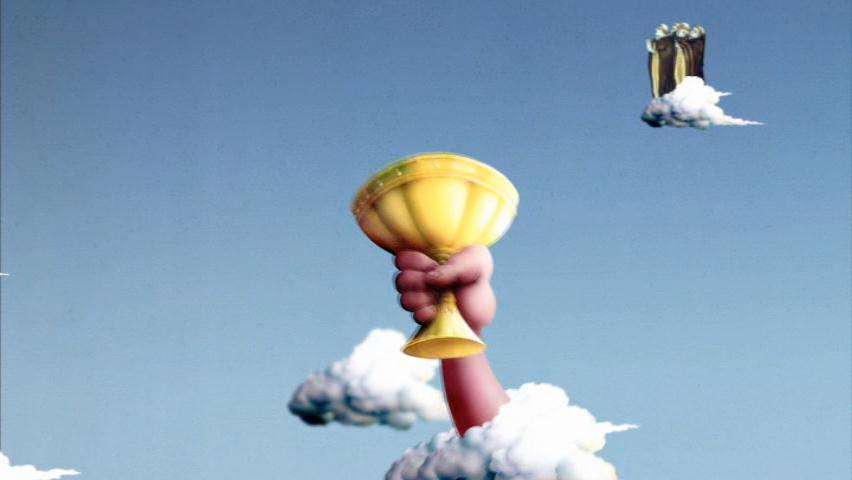
\includegraphics[width=1.0\linewidth]{grail}
%\captionof{figure}{\color{HoGentAccent5} He hasn't got shit all over him. The nose? Where'd you get the coconuts? What do you mean? We shall say 'Ni' again to you, if you do not appease us}
%\end{center}\vspace{1cm}

%------------------------------------------------



\color{HoGentAccent1} 
\section*{Conclusies}
\color{black}
\begin{center}\vspace{1cm}
    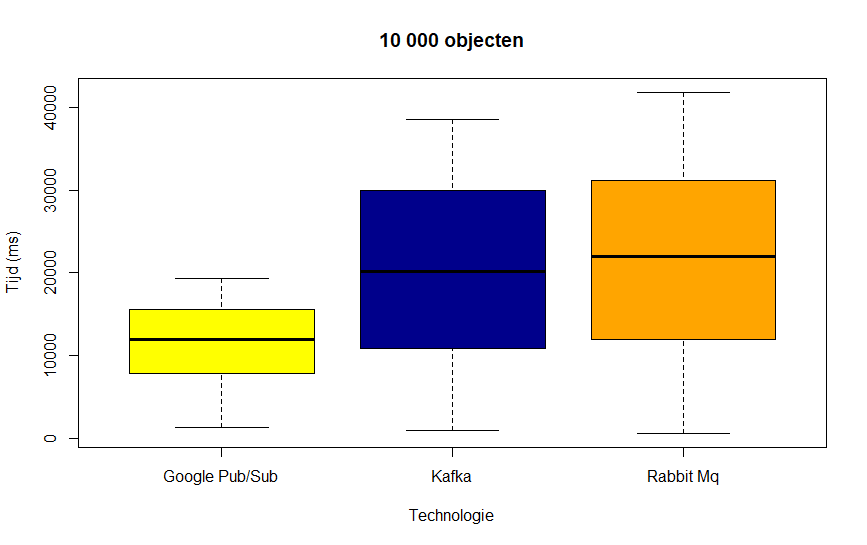
\includegraphics[width=200mm]{10000Boxplot}
    \captionof{figure}{\color{HoGentAccent5} Vergelijking bij 10 000 objecten}
\end{center}\vspace{1cm}
\begin{center}\vspace{1cm}
    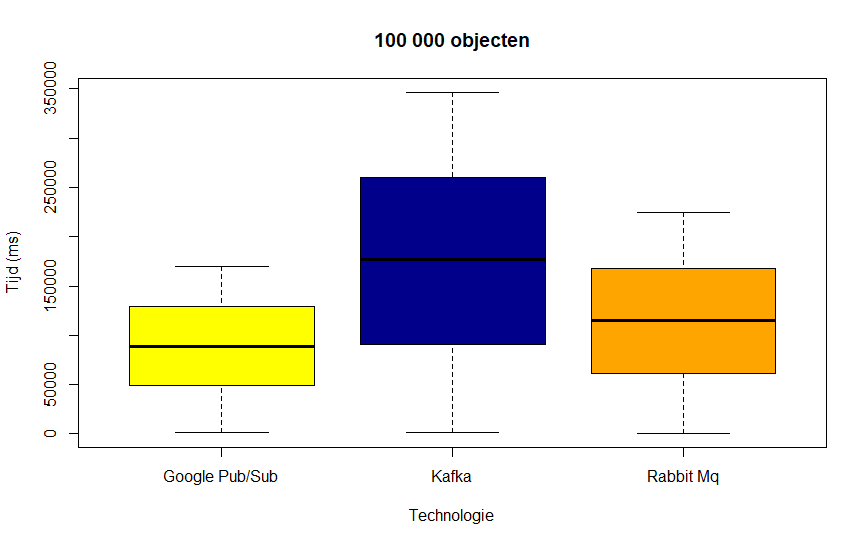
\includegraphics[width=200mm]{100000Boxplot}
    \captionof{figure}{\color{HoGentAccent5} Vergelijking bij 100 000 objecten}
\end{center}\vspace{1cm}
\begin{center}\vspace{1cm}
    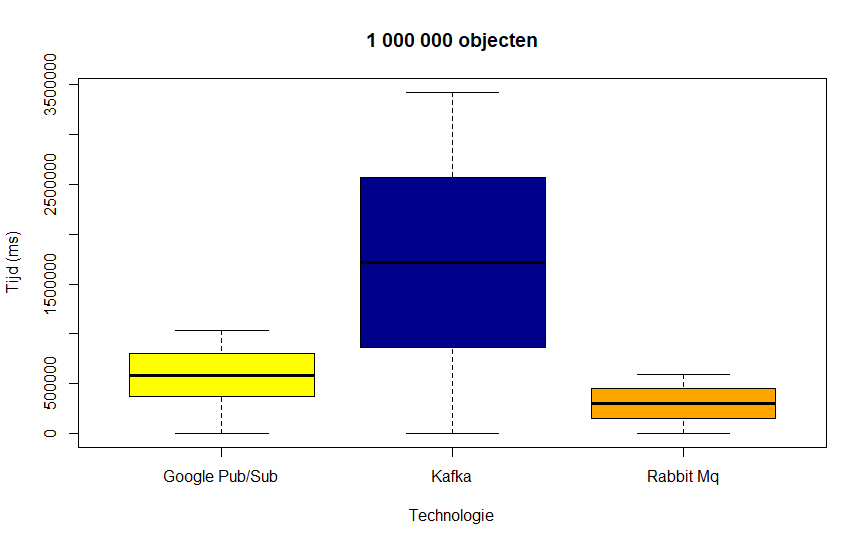
\includegraphics[width=200mm]{1000000Boxplot}
    \captionof{figure}{\color{HoGentAccent5} Vergelijking bij 1 000 000 objecten}
\end{center}\vspace{1cm}

\begin{center}\vspace{1cm}
    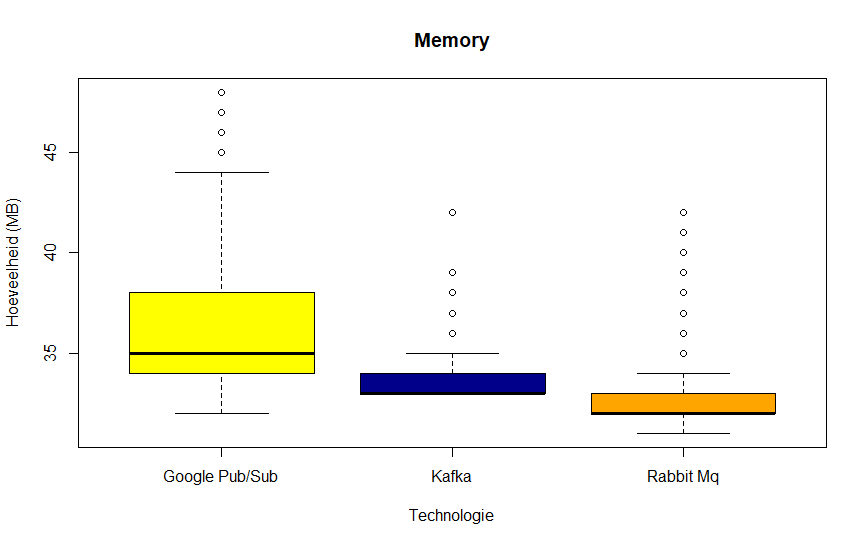
\includegraphics[width=200mm]{memory}
    \captionof{figure}{\color{HoGentAccent5} Vergelijking geheugen}
\end{center}\vspace{1cm}
Wanneer snelheid voor een bedrijf het belangrijkste is, dan lijkt Google Pub/Sub het beste. Tenzij je heel veel objecten hebt (meer dan 1 000 000) dan lijkt RabbitMq sneller te werken. Het geheugengebruik is het best bij RabbitMq maar Kafka doet het niet veel slechter. Bij Kafka ben je het meest zeker dat je effectief al je verzonden data meteen ontvangt. Hier slaagt RabbitMq het slechtste op.
Voor TVH specifiek lijkt het belangrijkste dat alle data zeker meteen ontvangen wordt. Omdat Kafka hierop het beste scoort en bijna de beste is op basis van geheugengebruik, lijkt Kafka de beste technologie om te gebruiken binnen dit bedrijf.
%----------------------------------------------------------------------------------------
%	FORTHCOMING RESEARCH
%----------------------------------------------------------------------------------------
\color{HoGentAccent1} 
\section*{Toekomstig onderzoek}
\color{black}

Als verder onderzoek zou je dit onderzoek meerdere keren kunnen uitvoeren om te bepalen hoe frequent verzonden data niet meteen aankomt. Een andere mogelijkheid is om de applicaties niet lokaal maar in de cloud te laten draaien. Op die manier ben je niet afhankelijk van een pc of laptop.


%----------------------------------------------------------------------------------------

\end{multicols}
\end{document}